% Template for Seminar Papers
% Research Group for Parallel Computing
% Vienna University of Technology

% Copyright (C) 2015-2016
% Sascha Hunold <hunold@par.tuwien.ac.at>
% version 1.0.2

\documentclass[DIV12,a4paper]{scrartcl}

\usepackage[utf8]{inputenc}
\usepackage[T1]{fontenc}

%\usepackage{fixltx2e} 
\usepackage{amsmath}  
\usepackage{amssymb} 
\usepackage{microtype} 
\usepackage{enumitem} 
\usepackage{booktabs} 
\usepackage{nag}       % Issues warnings when best practices in writing LaTeX documents are violated.
\usepackage{hyperref}
\usepackage{xspace}
\usepackage{graphicx}
%%%%%%%%%%%%%%%%%%%%%%%%%%%%%%%%%%%
%CUSTOM PACKAGES

\usepackage[backend=biber,style=ieee,mincitenames=1,maxcitenames=2]{biblatex}
\usepackage{algorithm}
\usepackage[noend]{algpseudocode}
\usepackage{xargs}
\usepackage[pdftex,dvipsnames]{xcolor}
\usepackage[colorinlistoftodos,prependcaption]{todonotes}
\usepackage[autostyle]{csquotes}

%%%%%%%%%%%%%%%%%%%%%%%%%%%%%%%%%%%
% ONLY CHANGE THE FOLLOWING MACROS

% your name
\newcommand{\studname}{Stefan Haider}

% your matrikel
\newcommand{\studmatrikel}{1125543}

% name of seminar
\newcommand{\seminarname}{Efficient Shared Memory Programming}

% title of your seminar paper
\newcommand{\seminartitle}{The Adaptive Priority Queue with Elimination and Combining}

% date when you hand in seminar paper
\newcommand{\spdate}{24. Feb. 2017}

% uncomment your choice
\newcommand{\sptopic}{Seminar aus Programmiersprachen}
%\newcommand{\sptopic}{Seminar aus Algorithmik}
%\newcommand{\sptopic}{Seminar aus Software Engineering}
%\newcommand{\sptopic}{Seminar aus Theoretischer Informatik}

% who is supervising
\newcommand{\spbetreuer}{Univ.Prof. Dr. Jesper Larsson Träff}
%%%%%%%%%%%%%%%%%%%%%%%%%%%%%%%%%%%
% CUSTOM CONFIGURATION

\addbibresource{progsem.bib}
\setcounter{tocdepth}{3}
\graphicspath{{graphics/}}

\widowpenalties 1 10000

%\newcommandx{\unsure}[2][1=]{\todo[linecolor=red,backgroundcolor=red!25,bordercolor=red,#1]{#2}}
%\newcommandx{\change}[2][1=]{\todo[linecolor=blue,backgroundcolor=blue!25,bordercolor=blue,#1]{#2}}
%\newcommandx{\info}[2][1=]{\todo[linecolor=OliveGreen,backgroundcolor=OliveGreen!25,bordercolor=OliveGreen,#1]{#2}}
%\newcommandx{\improve}[2][1=]{\todo[#1]{#2}}

\newcommand{\Continue}{\textbf{continue}}
\newcommand{\attr}{\ensuremath{\leftarrow} }
\newcommand{\nullvalue}{\ensuremath{\bot}}
\newcommand{\maxLvl}{\ensuremath{\mathrm{MaxLvl}}}
\newcommand{\maxInt}{\ensuremath{\mathrm{MaxInt}}}
\newcommand{\minInt}{\ensuremath{\mathrm{MinInt}}}

\begin{document}

% !TEX root = ../paper.tex

\pagestyle{empty}

\begin{titlepage}
\begin{center}

\includegraphics[scale=1]{TU_INF_Logo_gray}
\hfill

\includegraphics[width=1.7cm]{final-logo-par}

\end{center}

\vspace*{1cm}

\begin{center}

\begin{Large}
Institut für Informationssysteme\\
Forschungsgruppe ``Parallel Computing'' (E184-5)\\
Prof. Dr. Jesper Larsson Träff\\[2cm]
\end{Large}

\begin{Huge}
\textbf{Seminararbeit}\\
\end{Huge}

\vspace*{1cm}

\begin{Large}
für ein \\
\sptopic{} \\
``\seminarname{}'' 
\end{Large}


\vspace*{2cm}

\begin{Large}
\textbf{``\seminartitle{}''}
\end{Large}

\vspace*{2cm}

\begin{Large}
\studname \\
Matrikelnummer: \studmatrikel\\[2cm]

Betreuer: \spbetreuer

\vspace*{2cm}
\spdate \\

\end{Large}
\end{center}

\end{titlepage}


\cleardoublepage

% !TEX root = ../paper.tex

\section*{Main Literature Sources}

The following seminar report is based on the following research article:

\begin{enumerate}
	\item \AtNextCite{\defcounter{maxnames}{999999}}\fullcite{calciu_adaptive_2014}
\end{enumerate}



\clearpage

% !TEX root = ../paper.tex

\section*{Erkl\"arung zur Verfassung der Arbeit}

\vspace*{3ex}

\noindent
Hiermit erkl\"are ich, dass ich diese Arbeit selbst\"andig verfasst habe, dass ich die verwendeten Quellen und Hilfsmittel vollst\"andig angegeben habe und dass ich die Stellen der Arbeit -- einschließlich Tabellen, Karten und Abbildungen --, die anderen Werken oder dem Internet im Wortlaut oder dem Sinn nach entnommen sind, auf jeden Fall unter Angabe der Quelle als Entlehnung kenntlich gemacht habe.\\[5ex]

\noindent
\rule{8cm}{.5pt} \\
Wien, \spdate \\
\studname


\clearpage

\tableofcontents

\cleardoublepage

\pagestyle{plain}

\setcounter{page}{1}

% !TEX root = ../paper.tex

% !TEX root = ../paper.tex

\section{Introduction}

\unsure{Give context to the paper.. long intro.. skip some of the main part}

A priority queue is a data structure for storing elements with associated keys. The keys represent priorities. Priority queues can be implemented in two forms: max-priority queues and min-priority queues. The latter one is the form that is considered in this paper.
Typically a min-priority queue exports two operations: \texttt{add()}, for inserting an item into the priority queue, and \texttt{removeMin()} for removing the element with the minimum priority. \citeauthor{cormen_introduction_2009} describe other typical operations of a priority queue like: \texttt{minimum()} for retrieving without removing the minimum-priority-element, and \texttt{decreaseKey()} for decreasing the key of the given element to a given value.
(Parallel) priority queues are often used for resource management in schedulers, for event simulations, or as data structures in graph-algorithms (e.g. Dijkstra's shortest path algorithm, or Prim's minimum spanning tree algorithm) \cite{cormen_introduction_2009}.

\subsection{Prior Work}

The first parallel priority queues implementations were based on heaps and linked lists as it can be seen in the study by \citeauthor{ronngren_comparative_1997} \cite{ronngren_comparative_1997}, parallel priority queue algorithms based on skiplists were proposed later by \citeauthor{shavit_scalable_1999}. This first implementation deals with bounded range priority queues as found in operating system schedulers. Such queues provide a fixed range of priorities. The algorithm uses coarse-grained locking for synchronizing concurrent \texttt{removeMin()} operations and is based on the concurrent skiplist by \citeauthor{pugh_concurrent_1990} as described in \cite{pugh_concurrent_1990} \cite{shavit_scalable_1999}.

\citeauthor{lotan_skiplist-based_2000} proposed a general purpose priority queue based on \citeauthor{pugh_concurrent_1990}'s concurrent skiplist. Each element has a flag to mark it as deleted. A delete pointer points to the current minimum priority element. Each \texttt{deleteMin()} operation traverses the skiplist until it finds a non marked element. The element is marked and afterwards deleted from the skiplist \cite{lotan_skiplist-based_2000}.

A lock-free priority queue based on a skiplist was introduced by \citeauthor{sundell_fast_2003}. They use different atomic primitive operations like Test-And-Set~(TAS), Fetch-And-Add~(FAA) and Compare-And-Swap~(CAS) to make their priority queue lock-free. For deletion, they use previously unused bits of the pointers in the skiplist to mark the node as deleted\cite{sundell_fast_2003}.

\citeauthor{shavit_elimination_1997} introduced the concept of elimination. This technique allows opposing operations to be coupled together by exchanging data via a small elimination datastructure. The distributed datastructure remains unchanged \cite{shavit_elimination_1997}.

The paper by \citeauthor{hendler_flat_2010} introduced the concept of flat combining. This concept is the opposing strategy to use fine-grained locking to keep the critical region small, as it uses a global lock on the datastructure. All access requests are combined and executed all at once before releasing the lock. The benefit of this approach is the reduced synchronization overhead and the reduced traffic through cache invalidations \cite{hendler_flat_2010}.

\subsection{Contributions}

\citeauthor{calciu_adaptive_2014} developed a priority queue based on skiplists. They utilize the skiplists \enquote{capability for operation-batching and disjoint-access parallelism} \cite[407]{calciu_adaptive_2014}.

The elimination algorithm allows \texttt{add()} operations with keys smaller than the current queues minimum to eliminate with \texttt{removeMin()} operations. The idea of aging operations also allows \texttt{add()} operations to participate in elimination(if the key is below a certain threshold), even if they are not allowed to eliminate yet.

\texttt{RemoveMin()} operations are combined and delegated to a server thread. This thread is operating on the separate first part of the priority queue and serves every \texttt{removeMin()} and \texttt{add()} operation that is not eliminated.

\texttt{Add()} operations with keys over the threshold mentioned above do not use elimination. They are inserted into the skiplist directly. As inserting elements sequentially would be ineffective the skiplist is split into two parts. The first part is only operated by the server thread. The second part is accessed by all threads in parallel.

This design reduces contention through batched sequential \texttt{removeMin()} and \texttt{add()} (with small keys) operations, by using elimination, and by using parallel \texttt{add()} (with big keys) operations. 

\citeauthor{calciu_adaptive_2014} also implemented the algorithm by using hardware transactional memory instead of locks. The goal of this approach is to further increase performance and to simplify the implementation \cite{calciu_adaptive_2014}.

\subsection{Basics}

\change{Explain skiplist}

\change{Explain hardware transactional memory}

% !TEX root = ../paper.tex

\section{Design}

The priority queue implementation by \citeauthor{calciu_adaptive_2014} exports the two operations \texttt{add()} and \texttt{removeMin()}. It is based on a skiplist which is split into two parts as it can be seen in figure~\ref{fig:pqe}. The elements in the skiplist are buckets having associated keys accessible via \texttt{bucket.key}. \texttt{RemoveMin()} and \texttt{add()} operations with small keys are served by the sequential part, while \texttt{add()} operations with keys over a certain threshold are executed on the parallel part. The last element of the sequential part is referred to as \texttt{lastSeq} \cite{calciu_adaptive_2014}.

\begin{figure}[htb]
	\centering
	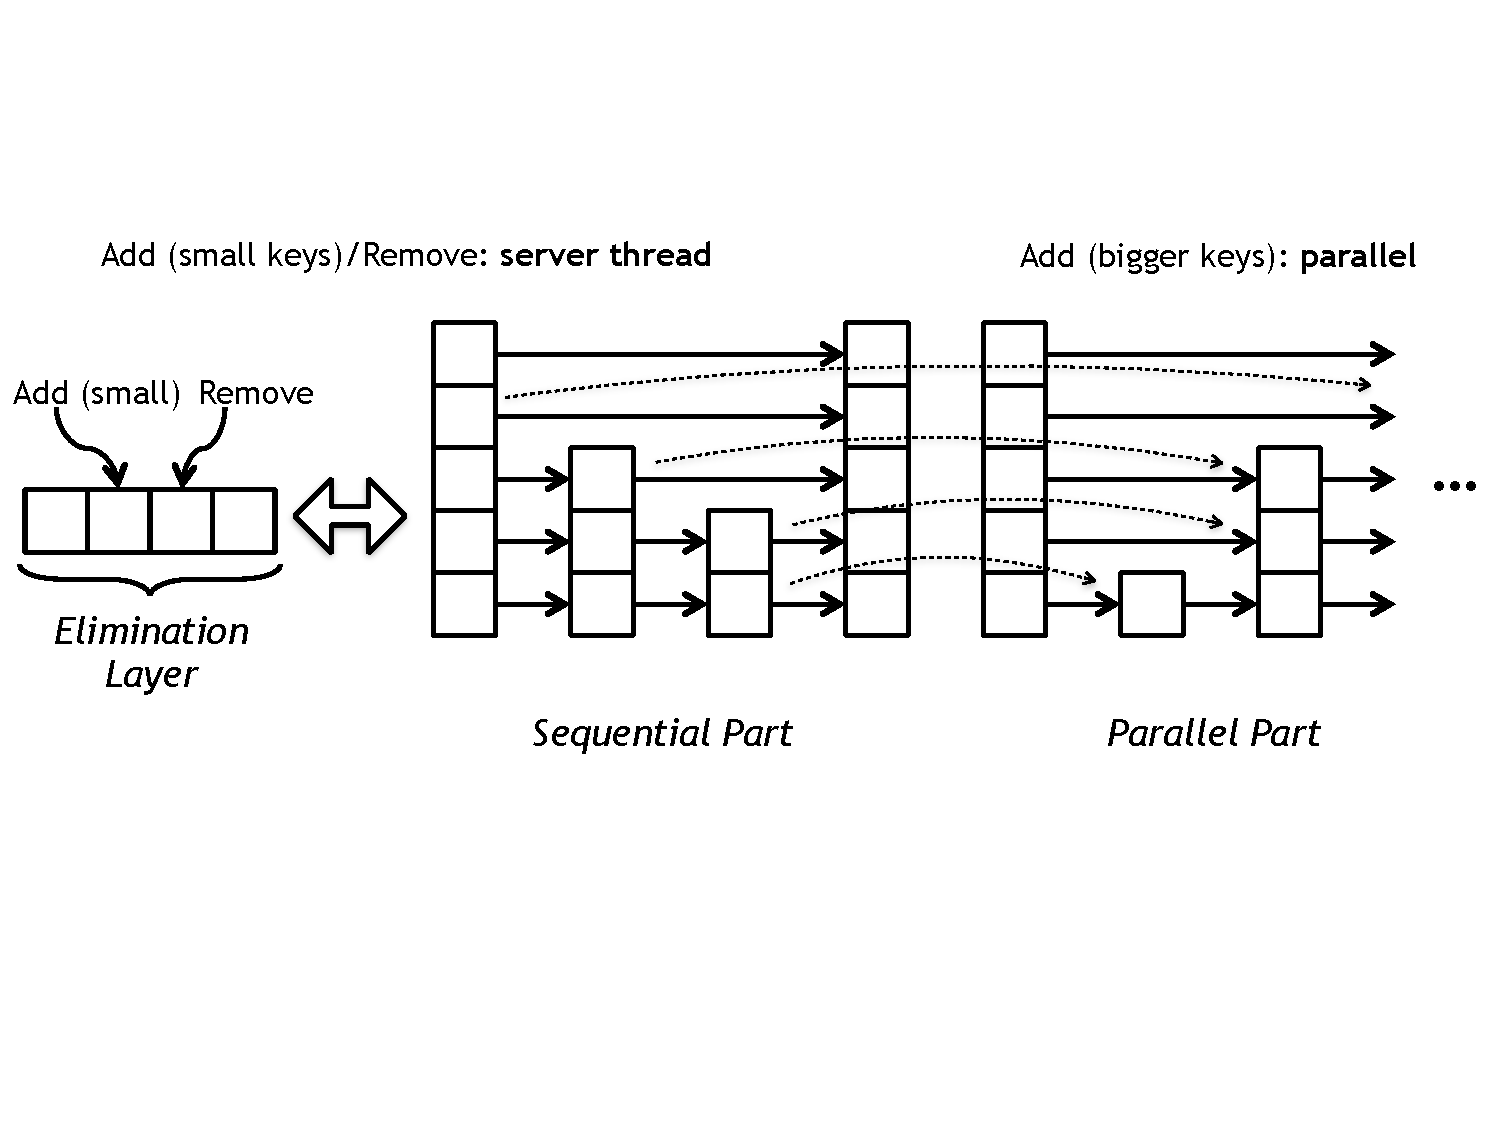
\includegraphics[width=0.9\textwidth]{graphics/pqe.pdf}
	\caption{Skiplist design \cite{calciu_adaptive_2014}.}
	\label{fig:pqe}
\end{figure}

\paragraph{Add()}

A thread executing \texttt{add($v$)} on the priority queue decides to insert the element concurrently into the parallel part if $v > \texttt{lastseq.key}$. Otherwise, the element is put into the elimination array as and add request. If the element becomes eligible for elimination ($v < \texttt{minValue}$) the operation can eliminate with any \texttt{removeMin()} occurring, otherwise the operation will be executed by the server thread \cite{calciu_adaptive_2014}.

\paragraph{RemoveMin()}

operations try to eliminate with an \texttt{add()} operation from the elimination array. If no operation is available, the thread writes a remove request to the array. It then gets either eliminated by a suitable \texttt{add()} operation or served by the server thread \cite{calciu_adaptive_2014}.

\subsection{Elimination and Combining}

Elimination allows operations to cancel each other out without accessing the shared datastructure. This reduces contention on the priority queue itself and therefore increases parallelism and scalability. The priority queue allows \texttt{removeMin()} operations to eliminate \texttt{add()} operations with keys smaller than \texttt{minValue} and vice versa. An array with a fixed size is used to store data the operations need to exchange \cite{calciu_adaptive_2014}.

\subsubsection{Elimination Array}

64 bit array slots are used to store a 32-bit value or one of the predefined opcodes as well as a unique stamp for every operation. Valid opcodes are: \texttt{EMPTY}, \texttt{REMREQ}, \texttt{INPROG}, and \texttt{TAKEN}. The values corresponding to these opcodes are not allowed to be used as values in the priority queue. These opcodes have following meaning:

\begin{description}
	\item[EMPTY] signals an unused slot of the elimination array.
	\item[REMREQ] is used by threads during a \texttt{removeMin()} operation to signal other threads the possibility to eliminate or instruct the server thread to remove an item from the priority queue.
	\item[INPROG] signals an adding thread that the server thread started to process the value that it wanted to add.
	\item[TAKEN] signals an adding thread that the value has been processed either by the server thread or a removing thread.
\end{description}

Other values stored in the elimination array are actual values being exchanged. The unique stamp also stored with the opcode/value is used for recognizing changes to the values stored in the elimination array and therefore ensuring linearizablity which will be covered in detail in section~\ref{sec:linearizablity}. This stamp is obtained by the thread ID and a thread-local operation counter \cite{calciu_adaptive_2014}.

\subsubsection{Operations and Elimination}

State transitions in the elimination array follow the state machine shown in figure~\ref{fig:combining-state}. Every slot is initially \texttt{EMPTY} with a stamp of 0. 

\begin{figure}[htb]
	\centering
	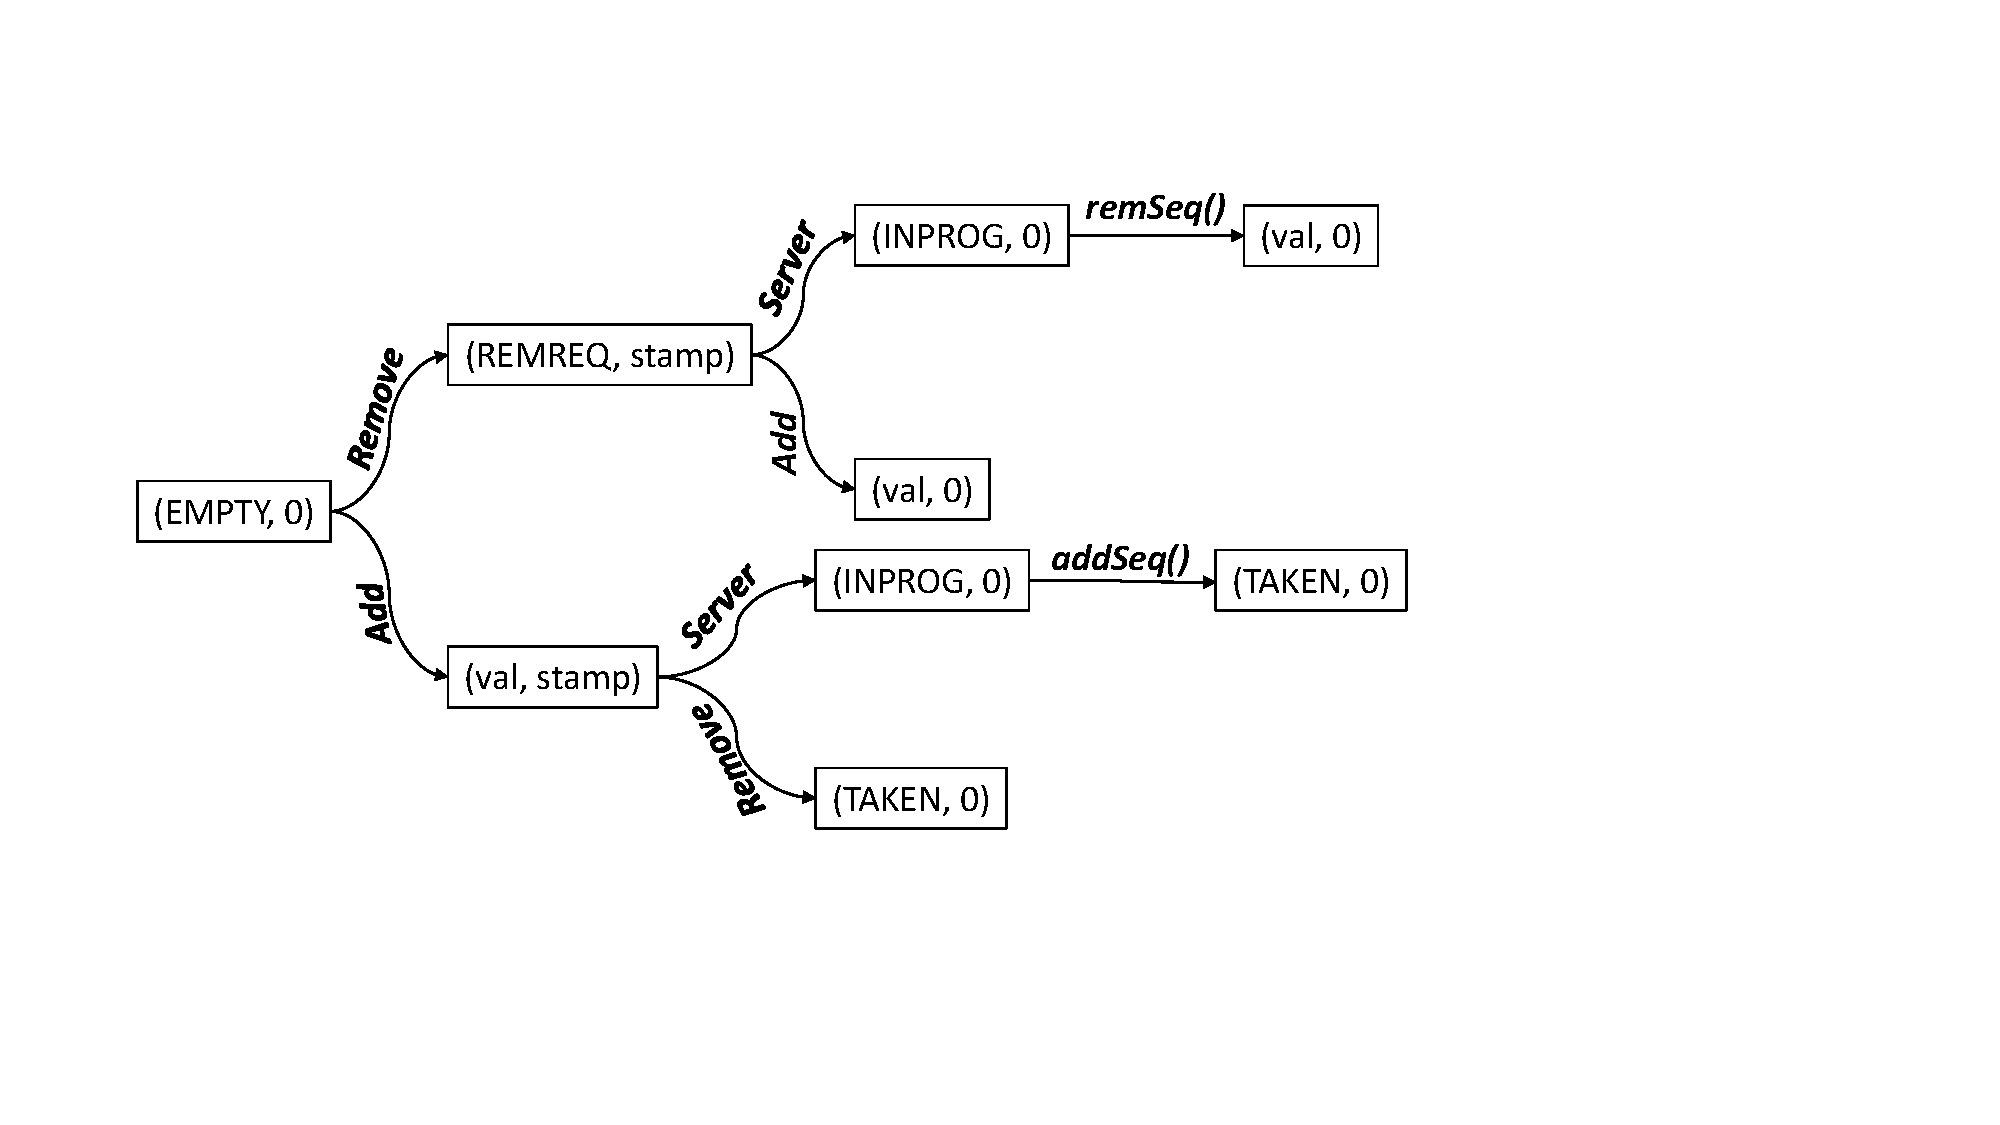
\includegraphics[width=0.9\textwidth]{graphics/combining-state.pdf}
	\caption{Elimination array state transitions \cite{calciu_adaptive_2014}.}
	\label{fig:combining-state}
\end{figure}

\paragraph{Add()} A thread trying to add a \texttt{key} (where $\texttt{key} < \texttt{minValue}$) iterates through all slots of the elimination array to find a \texttt{REMREQ} opcode. If it finds one and additionally $\texttt{key} < \texttt{minValue}$, the tread uses \texttt{CAS} to write its value including a stamp into this slot. If multiple attempts fail, the thread instead writes its value into a slot marked as \texttt{EMPTY} and waits for another or the server thread to use the value and change the opcode to \texttt{TAKEN}. The code for this operation can be found in the appendix in algorithm~\ref{alg:add} \cite{calciu_adaptive_2014}.

\paragraph{RemoveMin()} A thread removing an element from the priority queue iterates through the elimination array until it finds a value or an \texttt{EMPTY} slot in the elimination array. If the stamp of this value is greater than zero, it is checked whether the value is smaller than \texttt{minValue}, otherwise a non positive stamp indicates a value to respond to another \texttt{REMREQ}. In the case of the value being a current minimum of the priority queue the thread uses \texttt{CAS} to replace the value with \texttt{TAKEN}. In the case of finding an empty slot first, a \texttt{REMREQ} with a unique stamp is posted to this slot. Then the thread waits for another thread to eliminate this remove request or the server thread to actually remove one element from the priority queue and post it to this slot of the elimination array. The code for this operation can be found in the appendix in algorithm~\ref{alg:removeMin} \cite{calciu_adaptive_2014}.

\paragraph{Server Thread} The dedicated server thread is implemented to ensure progress of all threads as not all remove requests and add operations eliminate. The server thread collects all add and remove requests and executes them sequentially on the sequential part of the skiplist. To keep the implementation linearizable the server thread first swaps the value or remove request with \texttt{INPROG}. After the insertion \texttt{TAKEN} is written to the according slot, for removes the value with stamp 0 is written to the slot. The code for this operation can be found in the appendix in algorithm~\ref{alg:Execute} \cite{calciu_adaptive_2014}.

\subsection{Skiplist Operations}

The priority queue operations \texttt{add()} and \texttt{removeMin()} use the operations described in this section to manipulate the skiplist.

\subsubsection{Sequential Part}

The \texttt{addSeq()} and \texttt{removeSeq()} operations are just straight forward skiplist operations as they do not have to deals with any synchronization mechanism. The code for \texttt{removeSeq()} is shown in algorithm~\ref{alg:RemoveSeq} \cite{calciu_adaptive_2014}.

\subsubsection{Parallel Part addPar()}

The \texttt{addPar()} operation relies on a Single-Writer-Multi-Reader lock to not manipulate any pointers while head-moving operation are running. To keep the critical section as short as possible this operation first performs a \texttt{cleanFind()} as seen in algorithm~\ref{alg:CleanFind}. It searches for the position to insert the element, then acquires the read lock, and checks a timestamp variable manipulated through locking. If the checked timestamp changed between the successful \texttt{find()} and the check within the critical section the operation has to retry from the start. The code is shown in algorithm~\ref{alg:AddPar} \cite{calciu_adaptive_2014}.

\subsubsection{Head-Moving Operations}

The head-moving operations are responsible for moving the boundary between the sequential and the parallel part of the skiplist. At the beginning of such a operation a write-lock is acquired to keep other threads from adding elements in parallel while the boundary is manipulated.

\paragraph{moveHead()}

The \texttt{moveHead()} operation is used to extract a new sequential part from the skiplist if a remove request cannot be served because of an empty sequential part. At first the algorithm decides on how many elements should be moved to the sequential part. The number changes adaptive between $2^3$ and $2^{16}$. If more than $N$ insertions were performed in the sequential part since the last \texttt{moveHead()} was performed, the number of elements to move is doubled, if less than $M$ are inserted then the number is halved. The code is shown in algorithm~\ref{alg:MoveHead} \cite{calciu_adaptive_2014}.

\paragraph{chopHead()}

The \texttt{chopHead()} operation is called if no remove operations have been performed in a while. This operation relinks the sequential and the parallel part to form a fully parallel skiplist. The code is shown in algorithm~\ref{alg:ChopHead} \cite{calciu_adaptive_2014}.

\subsection{Hardware Transactions}

\subsubsection{Head-Moving Operations}

\subsubsection{addPar()}


% !TEX root = ../paper.tex

\section{Linearizablity}
\label{sec:linearizablity}

Linearizability as defined by \citeauthor{herlihy_linearizability:_1990} is a widely used correctness condition for concurrent objects. Linearizability guarantees that each operation appears to have an atomic effect at some point between its invocation and response. This point is typically referred to as linearization point. Combinations of linearizable operations are still linearizable which leads to the definition of a linearizable object. An object is linearizable, if each sequence of operations on this object is linearizable \cite{herlihy_linearizability:_1990}.

For the priority queue to meet the desirable linearizability condition it remains to show that each operation is linearizable. 

\subsection{Skiplist Operations}

\paragraph{AddPar() and AddSeq()}

both have their linearization point at the moment the element is added to the bottom level of the skiplist. The only exception is the insertion of a value that is smaller than \texttt{minValue}. In this case the \texttt{minValue} has to be updated. If there is a sequential part, this is done by the server thread, otherwise the performing thread retries until it succeeds or another thread updates it to an even smaller value  \cite{calciu_adaptive_2014}.


\paragraph{MoveHead() and ChopHead()}

both execute while holding the write lock, which means they execute without any thread interfering as no \texttt{addPar()} operation is allowed to run and the other sequential operations are only invoked by the server thread itself. These operations linearize when the lock is released \cite{calciu_adaptive_2014}.

\subsection{Elimination and Combining}

The unique stamps introduced in section~\ref{sec:eliminationArray} are necessary to avoid the ABA\footnote{\enquote{ABA is not an acronym and is a shortcut for stating that a value at a shared location can change from A to B and then back to A} \cite[185]{dechev_understanding_2010}.} problem. Without this stamp a thread performing an elimination could be interrupted by other threads using the same slot without him noticing it. This would result in an exchange of values with another thread than anticipated, which would break linearizability.

Figure~\ref{fig:correctness_elim} visualizes at which point in time two threads involved in an elimination linearize. A thread either inserting or removing a value has to check the exchanged value for being smaller than \texttt{minValue}. In that case the linearization point is at the time of this observation. Other interleaving operations could manipulate the \texttt{minValue} after this observation without breaking linearizability.

\begin{figure}
	\centering
	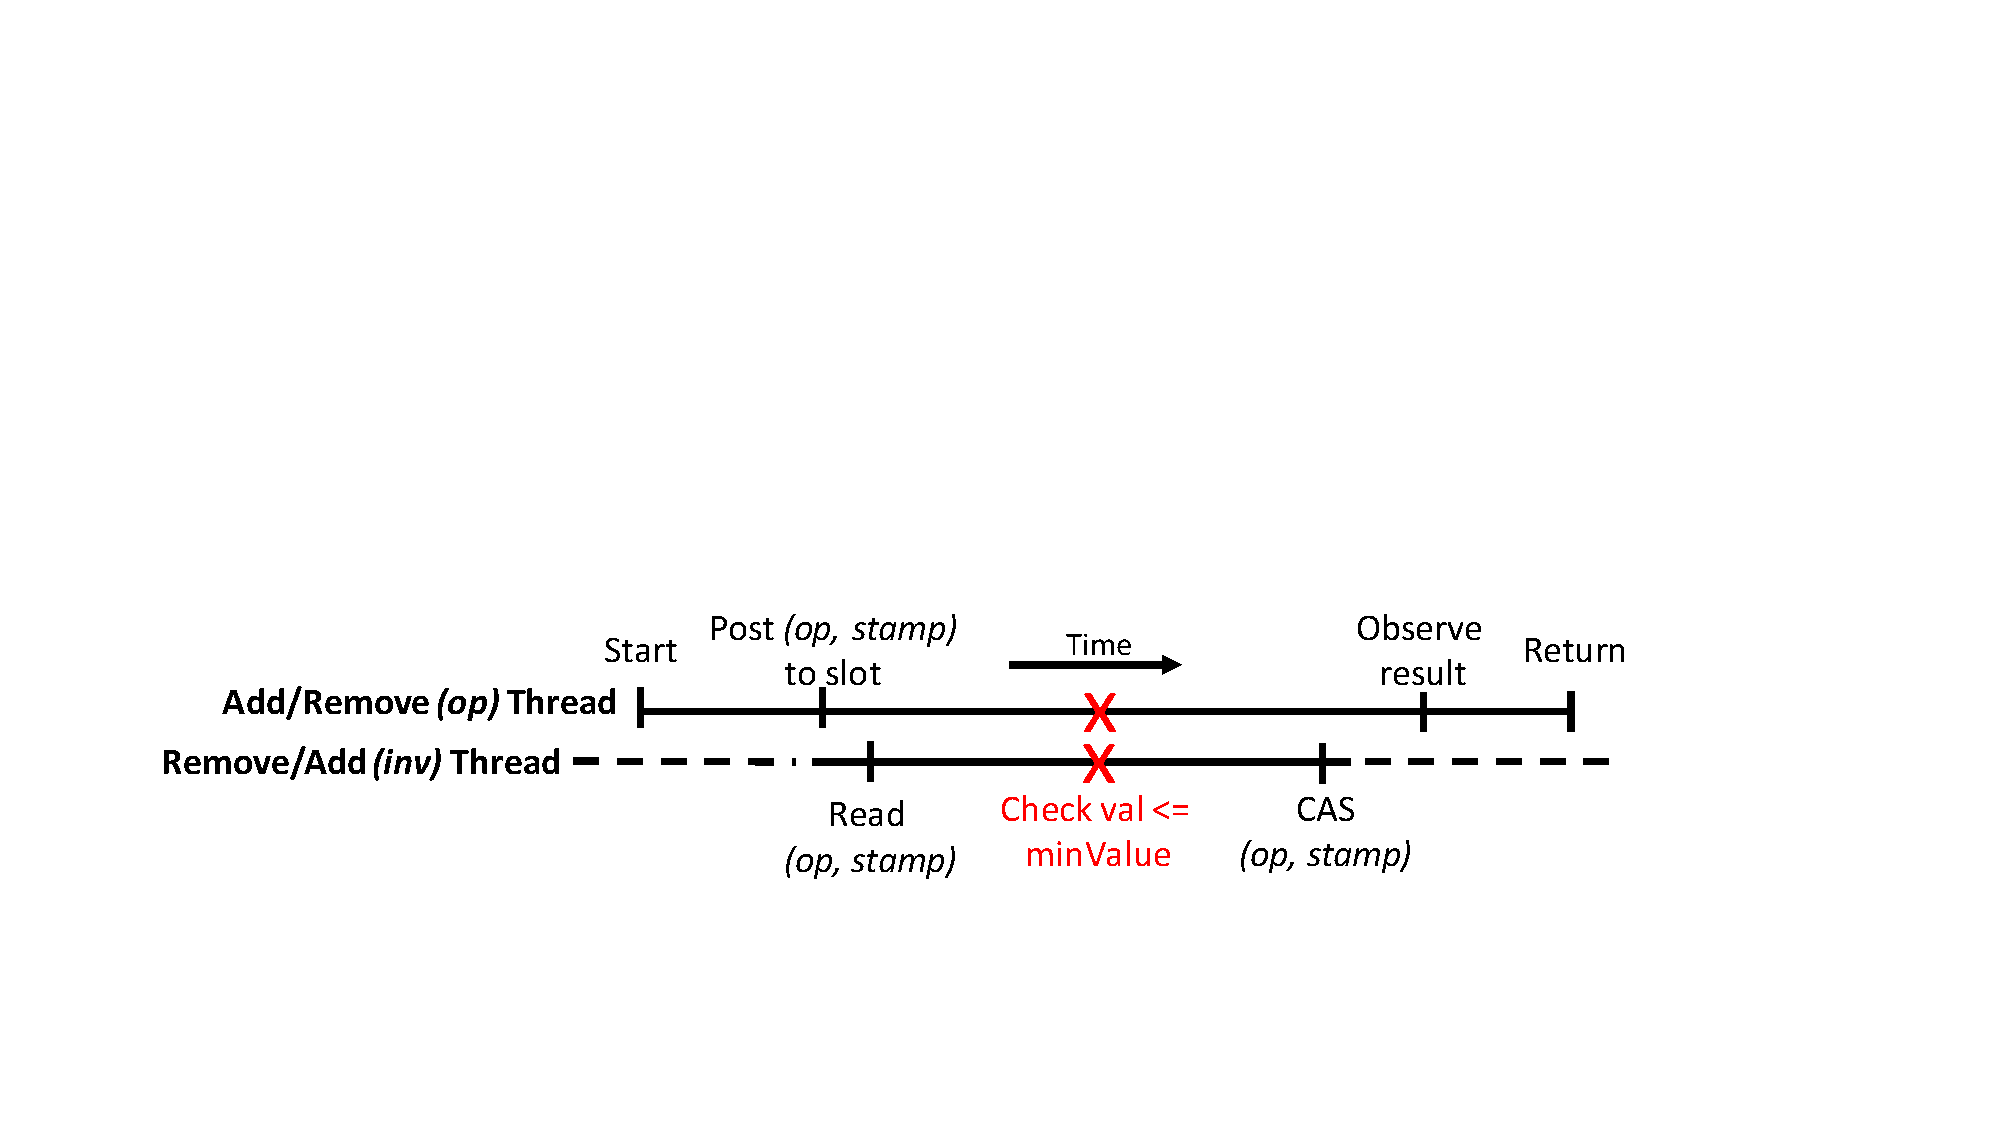
\includegraphics[width=0.9\textwidth]{graphics/correctness2.pdf}
	\caption{Execution of an \emph{op} thread and an \emph{inv} thread eliminating each other's operation. The linearization point is determined through the observation of the exchanged value being smaller than \texttt{minValue}. It is marked with a red X \cite{calciu_adaptive_2014}.}
	\label{fig:correctness_elim}
\end{figure}

Figure~\ref{fig:correctness_server} shows the point in time a thread linearizes while exchanging values with the server thread. The linearizability follows from the linearizability of the skiplist itself and the sequential execution on the skiplist \cite{calciu_adaptive_2014}. 

\begin{figure}[htb]
	\centering
	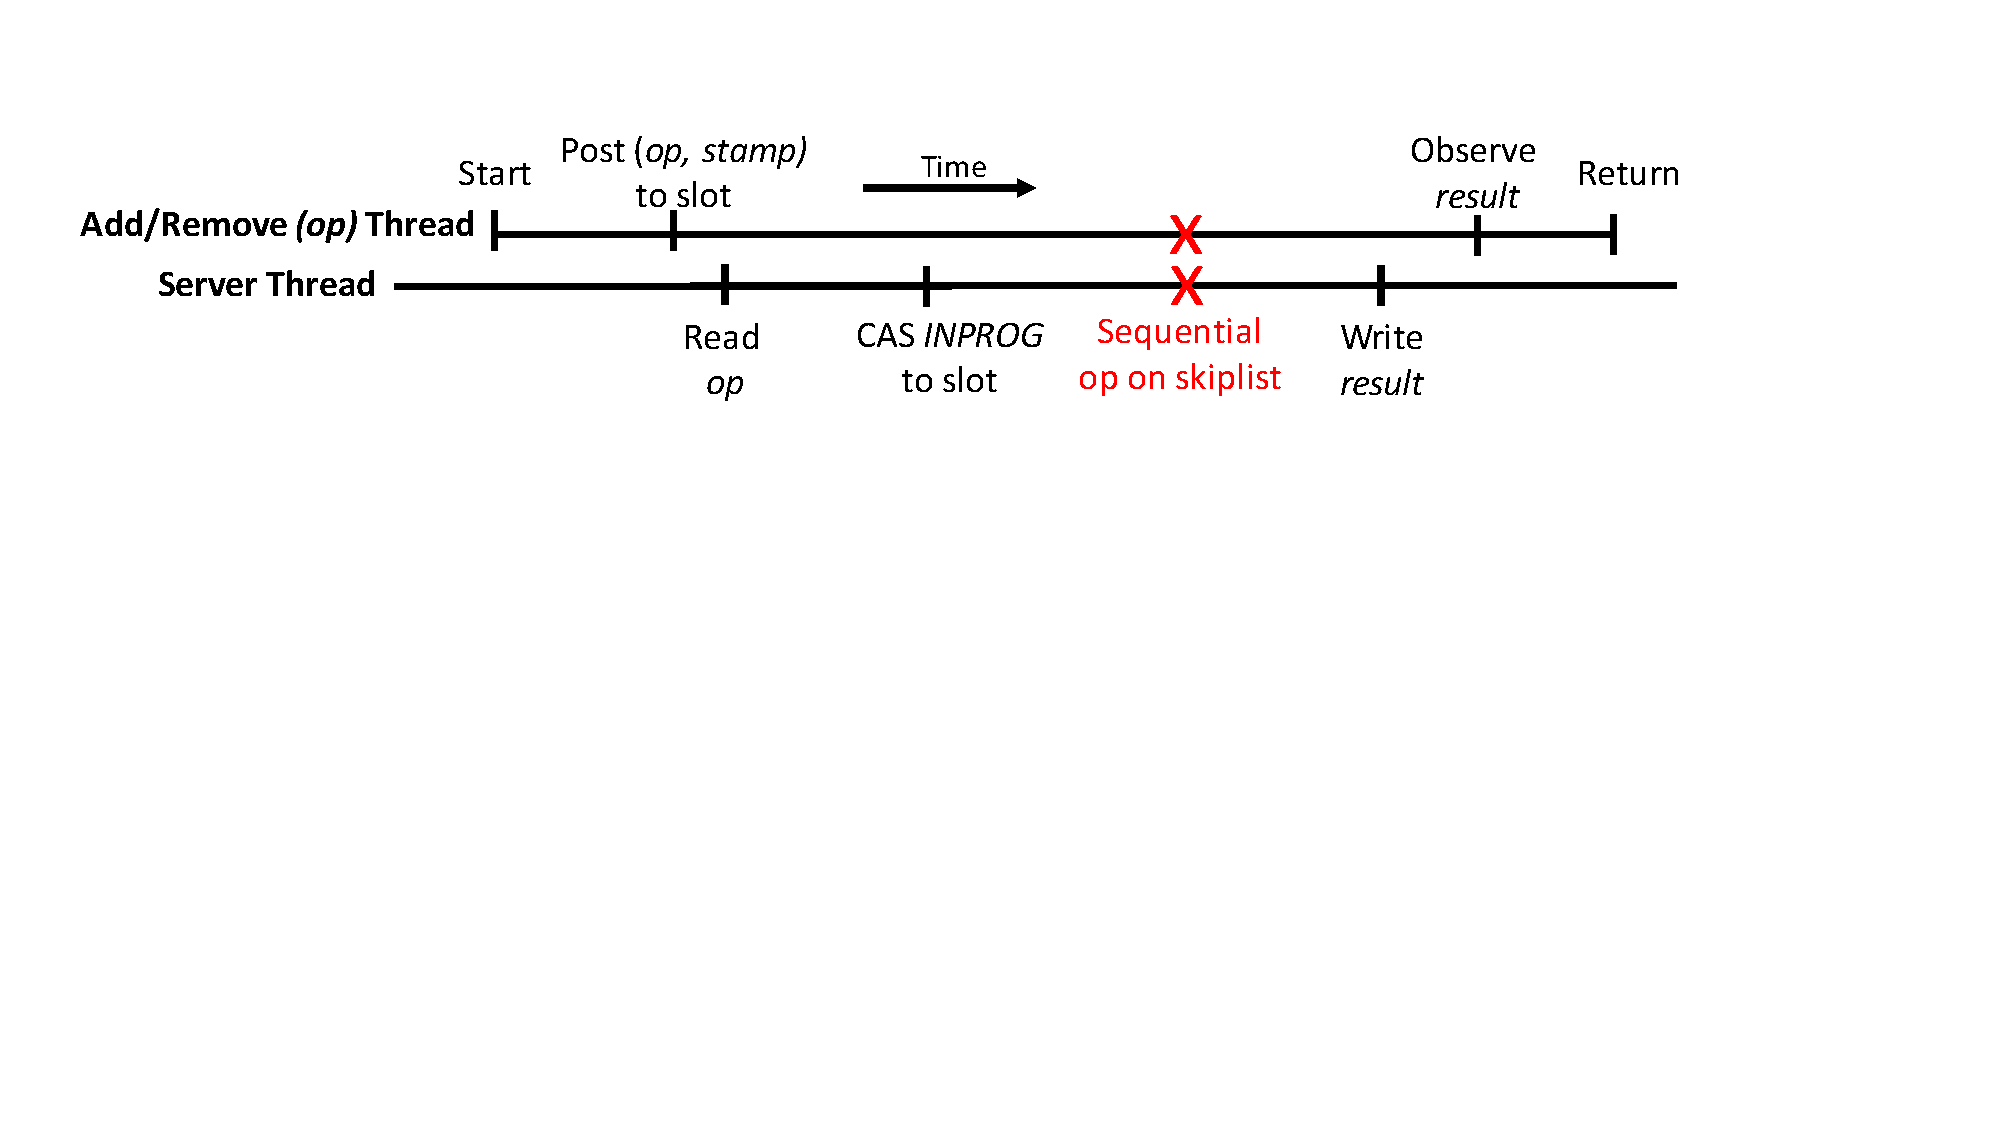
\includegraphics[width=0.9\textwidth]{graphics/correctness1.pdf}
	\caption{Execution of an \emph{op} having its operation served by the server thread. The linearization point is determined through the sequential operating server thread and is marked with a red X \cite{calciu_adaptive_2014}.}
	\label{fig:correctness_server}
\end{figure}

\subsection{Hardware Transactions}

When using transactions the linearization points are straight forward to determine. Each operation linearizes when the transaction completes successfully. 

% !TEX root = ../paper.tex

\section{Evaluation}

This section describes the result of both described algorithms. Although the   Newer priority queue implementation According to later published papers like \cite{braginsky_cbpq:_2016, } the performa



\subsection{Single-Writer-Multi-Reader Lock Implementation}

\subsubsection{Head-Moving Operations Overhead}

\subsection{Hardware Transactional Memory Implementation}

\subsubsection{Aborted Transaction Overhead}

\subsection{Comparison with succeeding papers}

C++ and compiled with a -O3 optimization level

\cite{braginsky_cbpq:_2016, } way better (used original code of this paper)

algorithm doesn't seem to scale much on multi socket machine, significant performance drop after useage of

AMD Opteron (TM) 6272
16-core processors, overall 64 threads. The machine was operated by Linux OS
(Ubuntu 14.04)

% !TEX root = ../paper.tex

\section{Conclusion}

\todo{We summarize the contribution of the papers and this seminar paper.}

\cleardoublepage

\printbibliography

\newpage
\appendix

% !TEX root = ../paper.tex

\section{Algorithm}

All the following algorithms are taken directly from the long version of the paper by \citeauthor{calciu_adaptive_2014-1} \cite{calciu_adaptive_2014-1}.

\begin{algorithm}[!htb]
	\caption{PQ::add(inValue)}
	\label{alg:add}
	\begin{algorithmic}[1]
		\If{inValue $\le$ skiplist.minValue}
		\State rep \attr MAX\_ELIM\_MIN
		\Else 
		\If{skiplist.addPar(inValue)}
		\State \Return $\mathbf{true}$
		\EndIf
		\State rep = MAX\_ELIM
		\EndIf
		
		\While{rep $> 0$}
		\State pos \attr $(id + 1) \% $ ELIM\_SIZE; (value, stamp) \attr 
		elim[pos]
		\If {value = REMREQ \textbf{and} (inValue $\le$ skiplist.minValue))}
		\If{CAS(elim[pos], (value, stamp), (inValue, 0))}
		\State \Return $\mathbf{true}$
		\EndIf
		\EndIf
		\State rep \attr rep $- 1$; inc(pos)
		\EndWhile
		
		\If{skiplist.addPar(inValue)}
		\State \Return $\mathbf{true}$
		\EndIf
		
		\While{$\mathbf{true}$}
		\State (value, stamp) \attr elim[pos]
		\If {value = REMREQ \textbf{and} (inValue $\le$ skiplist.minValue))}
		\If{CAS(elim[pos], (value, stamp), (inValue, 0))}
		\State \Return $\mathbf{true}$
		\EndIf
		\EndIf
		\If {value = EMPTY}
		\If{CAS(elim[pos], (value, stamp), (inValue, uniqueStamp()))}
		\Repeat
		\State (value, stamp) \attr elim[pos]
		\Until{value = TAKEN}
		\State elim[pos] \attr (EMPTY, 0); \Return $\mathbf{true}$
		\EndIf    
		\EndIf
		\State inc(pos)
		\EndWhile
	\end{algorithmic}
\end{algorithm}

\begin{algorithm}[htb]
	\caption{PQ::removeMin()}
	\label{alg:removeMin}
	\begin{algorithmic}[1]
		\While{$\mathbf{true}$}
		\State pos \attr $(id + 1) \% $ ELIM\_SIZE; (value, stamp) \attr 
		elim[pos]
		\If {IsValue(value) \textbf{and} (stamp $> 0$) \textbf{and} (value 
		$\le$ skiplist.minValue))}
		\If{CAS(elim[pos], (value, stamp), (TAKEN, 0))}
		\State \Return value
		\EndIf
		\EndIf
		\If {value = EMPTY}
		\If{CAS(elim[pos], (value, stamp), (REMREQ, uniqueStamp()))}
		\Repeat
		\State (value, stamp) \attr elim[pos]
		\Until{value $\ne$ REMREQ \textbf{and} value $\ne$ INPROG}
		\State elim[pos] \attr (EMPTY, 0); \Return value
		\EndIf    
		\EndIf
		\State inc(pos)
		\EndWhile
	\end{algorithmic}
\end{algorithm}


\begin{algorithm}[htb]
	\caption{Server::execute()}
	\label{alg:Execute}
	\begin{algorithmic}[1]
		\While{$\mathbf{true}$}
		\For{$i$: 1 $\rightarrow$ ELIM\_SIZE}
		\State (value, stamp) \attr elim[i]
		\If{value = REMREQ}
		\If{CAS(elim[i], (value, stamp), (INPROG, 0))}
		\State min \attr skiplist.removeSeq(); elim[i] \attr (min, 0)
		\EndIf
		\EndIf
		\If {IsValue(value) \textbf{and} (stamp $> 0$)}
		\If{CAS(elim[i], (value, stamp), (INPROG, 0))}
		\State skiplist.addSeq(value); elim[i] \attr (TAKEN, 0)
		\EndIf    
		\EndIf
		\EndFor
		\EndWhile
	\end{algorithmic}
\end{algorithm}

\begin{algorithm}[!htb]
	\caption{SL::removeSeq()}
	\label{alg:RemoveSeq}
	\begin{algorithmic}[1]
		\If{minValue $=$ \maxInt}
		\State \Return \maxInt
		\EndIf
		\If{currSeq $=$ \nullvalue}
		\State moveHead()
		\EndIf
		\State key \attr currSeq.key
		\State currSeq.counter \attr currSeq.counter - 1
		\If{currSeq.counter $= 0$}
		\While{currSeq $\ne$ lastSeq}
		\State currSeq \attr currSeq.next[0]
		\If{currSeq.counter $> 0$}
		\State minValue = currSeq.key
		\State \Return key
		\EndIf
		\EndWhile
		\State moveHead()
		\EndIf
		\State \Return key
	\end{algorithmic}
\end{algorithm}

\begin{algorithm}[!htb]
	\caption{cleanFind($v$, preds, succs)}
	\label{alg:CleanFind}
	\begin{algorithmic}[1]
		\State $t$ \attr lock.timestamp \label{algFLT:checkstamp1}
		\State $b$ \attr find(headPar, $v$, preds, succs)
		\State lock.acquireR()
		\If{$t$ $<$ lock.timestamp} \label{algFLT:checkstamp2}
		\State lock.release()
		\State \Return $(\nullvalue, \mathbf{false})$
		\EndIf
		\State \Return $(b, \mathbf{true})$
	\end{algorithmic}
\end{algorithm}

\begin{algorithm}[!htb]
	\caption{SL::addPar($v$)}
	\label{alg:AddPar}
	\begin{algorithmic}[1]
		\If{$v$ $\le$ lastSeq.key}
		\State \Return \textbf{false}
		\EndIf
		\State $(b,r)$ \attr cleanFind($v$, preds, succs) \label{algAddPar:find}
		\If{$r$ = \textbf{false}}
		\State \textbf{restart} at line~\ref{algAddPar:find}
		\EndIf
		\If{$b \ne \nullvalue$} \label{algAddPar:incblock}
		\State Atomically increment $b$.counter
		\State lock.release()
		\State \Return \textbf{true}
		\EndIf
		\State $b$ \attr newNode($v$)
		\For{$i$: 1 $\rightarrow$ $b$.topLevel}
		\State $b$.next[i] \attr succs[i]
		\EndFor
		\If{\textbf{not} CAS(preds[0].next[0]: succs[0] $\rightarrow$ $b$)}
		\State lock.release()
		\State \textbf{restart} at line~\ref{algAddPar:find}
		\EndIf
		\Repeat
		\State $m$ \attr minValue
		\Until{$m \le v$ \textbf{or} CAS(minValue: $m \rightarrow v$)}
		\For{$i$: 1 $\rightarrow$ $b$.topLevel}
		\State $b$.next[i] \attr succs[i]
		\If{CAS(preds[i].next[i]: succs[i] $\rightarrow$ $b$)}
		\State \Continue
		\EndIf
		\State lock.release()
		\Repeat
		\State $(b,r)$ \attr cleanFind($v$, preds, succs)
		\Until{$r = \mathbf{true}$}
		\If{$b = \nullvalue$}
		\State lock.release()
		\State \Return \textbf{true}
		\EndIf
		\EndFor
		\State \Return \textbf{true}
	\end{algorithmic}
\end{algorithm}

\begin{algorithm}[!htb]
	\caption{SL::moveHead()}
	\label{alg:MoveHead}
	\begin{algorithmic}[1]
		\State $n$ is determined dynamically (see text)
		\State lock.acquireW()
		\State currSeq \attr \nullvalue
		
		\State pred \attr headPar
		\State curr \attr headPar.next[0]
		\State $i = 0$
		\While{$i < n$ \textbf{and} curr $\ne$ tail} \label{algMH:consume}
		\State i \attr i + curr.counter
		\If{currSeq = \nullvalue}
		\State currSeq \attr curr; minValue \attr curr.key
		\EndIf
		\State pred \attr curr; curr \attr curr.next[0]
		\EndWhile
		
		\If{$i = 0$}
		\For{$i: \maxLvl \rightarrow 0$}
		\State headPar[i], headSeq[i] \attr tail
		\EndFor
		
		\State lastSeq \attr headPar, minValue \attr \maxLvl
		\State lock.release()
		\State \Return \textbf{false}
		\EndIf
		
		\State lastSeq \attr pred
		
		\For{$i: \maxLvl \rightarrow 0$} \label{algMH:copyHead}
		\State headSeq[i] \attr headPar[i]
		\EndFor
		
		\State find(headSeq, lastSeq + 1, preds, succs) \label{algMH:unlink}
		
		\For{$i: \maxLvl \rightarrow 0$}
		\State preds[i].next[i] \attr tail
		\State headPar.next[i] \attr succs[i]
		\EndFor
		
		\State lock.release()
		\State \Return \textbf{true}
	\end{algorithmic}
\end{algorithm}

\begin{algorithm}[!htb]
	\caption{SL::chopHead()}
	\label{alg:ChopHead}
	\begin{algorithmic}[1]
		\If{currSeq = \nullvalue}
		\State \Return \textbf{false}
		\EndIf
		
		\State find(headSeq, lastSeq.key + 1, preds, \nullvalue)
		\State find(headSeq, currSeq.key, \nullvalue, succs)
		
		\State lock.acquireW()
		
		\For{$i: \maxLvl \rightarrow 0$}
		preds[i].next[i] \attr headPar.next[i]
		\EndFor
		
		\State lastSeq \attr headPar, currSeq \attr \nullvalue
		
		\For{$i: \maxLvl \rightarrow 0$}
		\State headPar.next[i] \attr succs[i] \textbf{if} succs[i] $\ne$ tail
		\EndFor
		
		\State lock.release()
		
		\State \Return \textbf{true}
	\end{algorithmic}
\end{algorithm}
\end{document}